\chapter{Conclusion and Outlook}
There is still an ongoing discussion about the feasibility, optimal sample and beam requirements of a proof-of-principle experiment of IDI at the nanoscale as well as about in which areas IDI can provide new information. More thorough theoretical studies , further improvements in experimental design and data analysis will be beneficial.


\paragraph{Developed tools for CDI/IDI experiments}
Both the GPU-accelerated simulation code and the reconstruction code developed for this thesis are open source\footnote{available under \url{https;//github.com/fzimmermann89/idi}} and will be used for planning and analyzing future IDI experiments. The simulation code allows to compare IDI and CDI experiments for the same sample, comparison for different samples and experimental parameters as shown in \fref{chap:simulation}.
The analysis code implements 2d, 3d and radial correlations for small and wide angle experiments with different normalization approaches as well as library of commonly needed auxiliary functions, such as dark and mask generation for pixel detectors, a new common mode correction with adaptive block sizes, photon counting procedures, different regression tools as well as tools for center finding and similar tasks.








\paragraph{Results of the Experiment}

The previously published results for the foil samples could be reproduced.
By using the presented preparation of nanoparticle samples in polymer matrix, aggregation could not be prevented, resulting in less pronounced features in higher $q$ instead of providing a structure factor similiar to non-interacting spheres as determined by the SAXS measurement. 



Furthermore, the Kossel line alignment tool with its graphical user interface allows easy analysis of the detector orientation for future experiments with strict alignment margins.



\paragraph{Experimental Improvements}



The posibility to run an IDI setup in parallel with other detectors would allow for a combination of IDI with CDI

Larger detectors

Short pulses

Element specific 

Recently, we performed an experiment using sub-1\,fs pulses at the CXI beamline at the LCLS free electron laser. In this experiment, three major improvements over the SACLA experiment were implemented: First, the shorter pulse length reduces the number of temporal modes and a shot-by-shot high resolution spectrometer allows for better filtering of the x-ray pulses by estimated pulse length and intensity. Second, the data was recorded in forward direction, solving the undersampling issue and reducing the spatial modes. And third, two new, signal optimized samples were chosen: Anodic aluminum oxide (AAO) membranes with regular spaced 20\,nm or 30\,nm wide pores, with are filled with Nickel or Vanadium using atomic layer deposition, creating an array of hexagonal placed 500\,nm long cylinders 60\,nm/100\,nm apart \cite{carina2019}. As the range of the order of the self-organizing pores is smaller than the total area used in the experiment, the simulated reconstruction shows rings (\fref{fig:outlook_aao}). 
The other sample is will be lithographically produced gratings with two diffferent pitches, 60\,nm  and 80\,nm \cite{mojarad2015}. For these samples, a simulation is shown in \fref{fig:outlook_grating}. Both samples combine the advantages of a single crystal sample (namely intense features) while providing more signal and requiring less accessible reciprocal space. 
Based on the simulations, it can be estimated, that a few hundred images taken with sub-fs pulses exciting 20\% of the atoms would suffice to reach a SNR of >3.
We were able to record full datasets on multiple samples. The data analysis of this experiment has not yet been completed and might result in the first experimental proof of using fluorescence intensity correlation for structural imaging at the nano-scale.  



\begin{figure}[p]
	\centering
	\begin{subfigure}[b]{0.50\textwidth}
		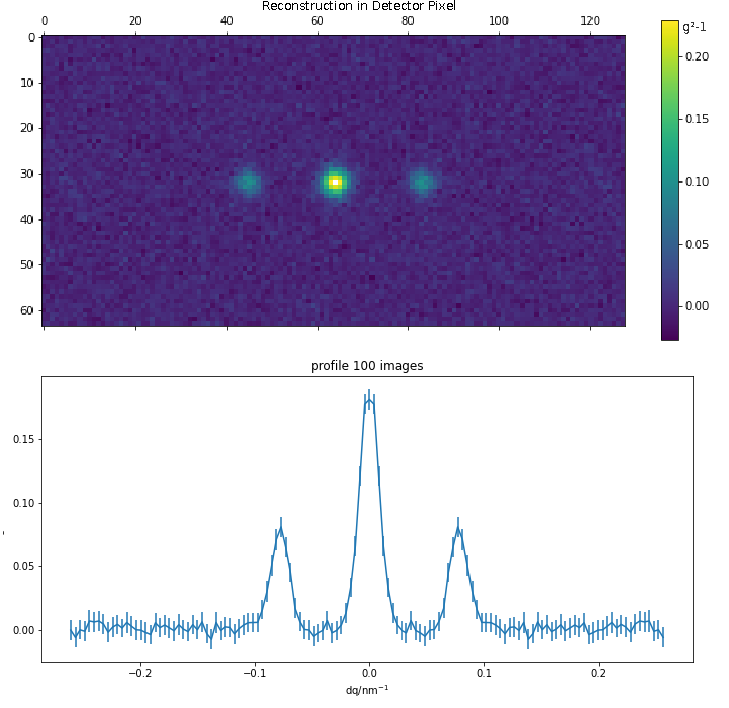
\includegraphics[width=\linewidth]{images/lv65simA.pdf}
		\caption{Nano-Grating}
		\label{fig:outlook_grating}
	\end{subfigure}
	\begin{subfigure}[b]{0.37\textwidth}
		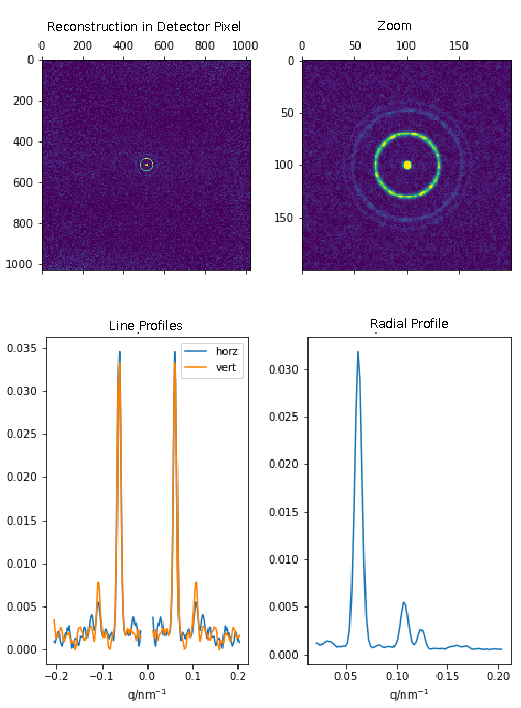
\includegraphics[width=\linewidth]{images/lv65simB.pdf}
		\caption{AAO membrane  }
		\label{fig:outlook_aao}
	\end{subfigure}
	\caption[Simulations in Preparation of LV65 Experiment]{Examples of simulations performed with the tools developed in this thesis in preparation of the LCLS free electron laser experiment LV65, which will use nano-gratings and AAO membranes with metal filled self-organized pores as samples for an IDI measurement. The simulations were used to chose an optimized sample geometry and to estimate the feasibility with respect to the expected SNR. The images shown are the calculated fluorescence intensity correlations between pixels of a quarter of an Jungfrau 4M detector placed at a distance of 70\,cm (grating) and 1\,m (membrane) respectively. The simulated grating has a pitch of 80\,nm, 40\,nm line width and 40\,nm thickness; 20\% excitation and 4 modes were simulated. The AAO membrane has and inter pore distance 105\,nm, the pores are filled with vanadium and 20\% excitation are assumed. For both samples, the average over 100 images is shown.}
\end{figure}


\paragraph{Using Incoherent Imaging for Online Beam Diagnostic}

Extending on the results obtained for both determining the focal volume as well as using the contrast to estimate the pulse length promises to be an useful diagnostic tool in future FEL experiments with ultra-short pulses and/or tight foci \cite{nakumura2020,inoue2019}. In the aforementioned LCLS experiment it has already been used successful during tuning to find the focal spot along the beam direction (see \fref{fig:outlook_vanadium} for examples of the online analysis).


\begin{figure}[p]
	\centering
	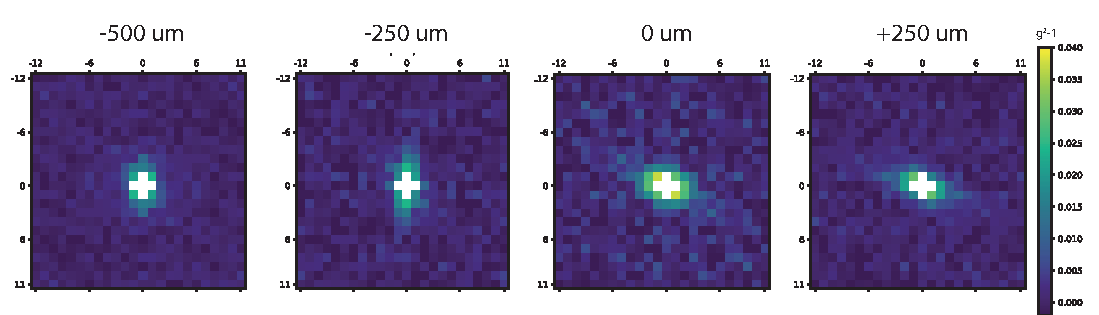
\includegraphics[width=\linewidth]{images/lv65_vanadium.pdf}
	\label{fig:outlook_vanadium}
	\caption[Focus finding using IDI]{Preliminary results of the $g^2(\vec{q})$ calculation of the fluorescence of a 4\,um vanadium foil, placed at 4 different positions along the X-ray beam at the CXI experimental hutch (LCLS, running in an experimental configuration for short pulse duration under 1\,fs \cite{subfs2017,argosecond}) using the "100 nm" KB focusing (optimal theoretical focus size 90\,nm x 150\,nm, theoretical beam divergence 2 mrad x 1 mrad) on one tile of a Jungfrau detector (75\,um pixelsize, placed 480\,mm downstream of the sample). The axis are in detector pixels. Shown are averages over ~2000 shots with minimal shot based filtering. The position captioned "0" was determined during the experiment as the focus based on these results, the other positions are 250\,um and 500\,um further downstream and 250\,um upstream (this position was previously determined as the focus by imprints).  Some astigmatism is visible.}
\end{figure}

\paragraph{Higher Order Correlations}

Extending the Hanbury-Brown and Twiss experiment to higher order correlations allows the usage of prior knowledge about the distribution of the spatial frequencies in the sample as an effective filter by fixing some terms in the correlation function at what certain positions termed  \textit{Magic Poisition}. A future application of this scheme in the analysis of the already recorded fluorescence patterns might lead to a significant increase in the SNR and resolution \cite{schneider2018,thiel2007}.